\subsection{Ablation Study}
\label{sec:evaluation-ablation}

We examine how individual rejection rules affect attack acceptance and
quantify the cost of cumulatively enabling lifecycle, handoff, provider,
and settlement validation.
The acceptance-rule controls and cost microbenchmark use separate
historical CPU measurements.

\noindent\textbf{Acceptance-rule sensitivity.}
For each selected attack, we compare the unmodified auditor's decision
with a control that converts rejection to acceptance when the first
failed relation matches the selected rule.
Each attack--decision configuration has 500 observations from five
fixtures, each repeated 100 times.
Table~\ref{tab:f-rule-gating} shows that the unmodified decisions reject
all tested call insertions, handoff modifications, evidence-splicing
attempts, and bill manipulations.
Relaxing the corresponding rejection rule accepts all 500 observations
in each case.
These controls show that the selected attack outcomes depend on distinct
rules in the final acceptance decision; they do not remove validation
code or resume auditing after the first failure.

\begin{table}[!t]
\centering
\caption{Post-audit acceptance-rule sensitivity (accepted/tested).}
\label{tab:f-rule-gating}
\footnotesize
\renewcommand{\arraystretch}{1.08}
\setlength{\tabcolsep}{3pt}
\begin{tabular*}{\columnwidth}{@{\hspace{3pt}}l@{\extracolsep{\fill}}lcc@{\hspace{3pt}}}
\toprule
\shortstack{\textbf{Relaxed}\\\textbf{rule}}
& \textbf{Attack}
& \shortstack{\textbf{Full}\\\textbf{decision}}
& \shortstack{\textbf{Relaxed}\\\textbf{decision}} \\
\midrule
$R_{\mathrm{life}}$ & Call insertion & 0/500 & 500/500 \\
$R_{\mathrm{hand}}$ & Handoff tampering & 0/500 & 500/500 \\
$R_{\mathrm{prov}}$ & Evidence splicing & 0/500 & 500/500 \\
$R_{\mathrm{set}}$ & Bill manipulation & 0/500 & 500/500 \\
\bottomrule
\end{tabular*}
\end{table}

\noindent\textbf{Incremental validation costs.}
The cost microbenchmark uses prebuilt evidence for eight calls and
32 lifecycle events.
Starting with an empty request-ID baseline, we cumulatively enable
lifecycle, bilateral-handoff, provider, and settlement validation.
Each configuration has five runs, with 100 warmups and 1,000 measured
executions per run, totaling 25,000 measured executions.
Timing covers these validation stages and payload-field selection;
authorization verification, evidence construction and signing, model
inference, serialization, persistence, ledger I/O, and proving are excluded.
Payload size is measured by canonical serialization after timing.

Figure~\ref{fig:f-component-costs}(a) reports increments computed within
matched runs.
The four stages add 6.03, 5.43, 2.91, and 2.34\,ms, respectively, yielding
a final four-stage cost of $16.70\pm0.11$\,ms and a selected payload of
32.22\,KiB.
Lifecycle and handoff validation account for 68.6\% of this time and
69.7\% of the selected payload.
Provider and settlement validation contribute the remaining 31.4\%
of time in this activation order.
These measurements characterize validation of prebuilt evidence;
the end-to-end and persisted-evidence costs are evaluated separately
in the preceding subsections.

\begin{figure}[!t]
\centering
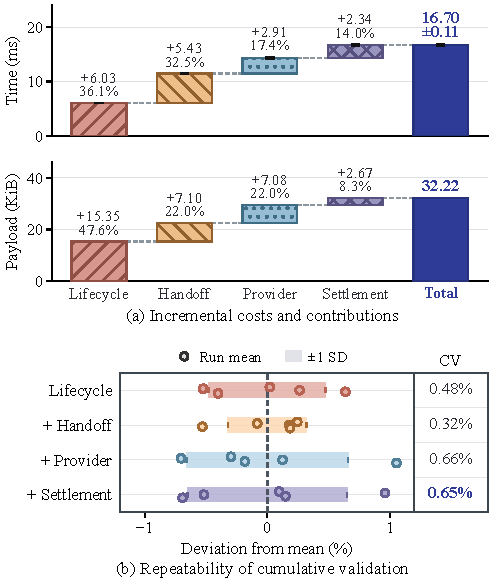
\includegraphics[width=\columnwidth]{f_component_waterfalls.pdf}
\caption{Costs and repeatability on prebuilt eight-call, 32-event fixtures.
(a) Waterfalls show mean paired increments and shares of the final total.
Time whiskers show sample SDs of the five run means for each cumulative
configuration. Totals include the 0.47\,$\mu$s/22\,B baseline.
(b) Points show signed percentage deviations of run means from their
cumulative configuration mean; shaded intervals span $\pm1$ sample SD.
CV is computed across the five run means.}
\label{fig:f-component-costs}
\end{figure}

\noindent\textbf{Repeatability.}
Figure~\ref{fig:f-component-costs}(b) shows all five run means for each
nonempty cumulative configuration.
Their coefficients of variation range from 0.32\% to 0.66\%, and the
largest absolute deviation from a configuration mean is 1.06\%.
For the final four-stage configuration, run means range from 16.59 to
16.86\,ms, with a CV of 0.65\%.
Selected payload sizes are identical across runs.
Thus, the validation microbenchmark exhibits low variation across its
five measured runs.
Appendix~\ref{app:f-ablation} provides the cumulative costs, matched
increments, individual run means, and aggregation definitions.
